\chapter{Implementation: Interpreter in Haskell}
Our implementation is an interpreter written by Haskell, which is a popular programming language. Haskell is also functional and has a static type system. Basically this will challenge us because Lua doesn't care types that much during coding. However, as a functional programming language, Haskell provides a fast runtime speed since it treats computations as a set of expressions of mathematical functions and this will possibly avoid mutable variables. 

Haskell also has simple memory allocation due to the research\cite{PIH}. As the trade off, there is no absolute meaning of ``global mutable variables'' such like global store of symbol table stack, and this would obviously differ in building interpreter between object-oriented language and functional language. Actually, this disadvantage would bring many troubles during the construction of the interpreter. We will talk about what those troubles are in the following sections.

What is more, although the interpreter is base on the syntax and semantic of FWLua, we want it to interpret the code of full version of Lua. Due to this, there would be a need of desugaring phase inside the interpreter. In the interpreter, we make this phase as a single, tiny tier in the interpreter, and create it as a single {\tt .hs} file in the program to keep the whole interpreter loose coupling.

In this chapter, we will mainly discuss about the whole structure of our interpreter, and paradigm of each element in the structure.

\section{Structure}
According to the reference\cite{WCAI}, we want our interpreter to be loose coupled\cite{looseC}. This term means that the program can be treat as several components. In addition, each component in the program is totally independent, with no, or few shared information or definitions against other parts. This term was introduced in case of keeping program adoptive, especially in designing compiler of interpreter. In other words, a loose-coupled interpreter can handle different kinds programming language by only changing specific key components in it.

Therefore, we design our interpreter being loose coupled by split it into several parts. Basically, there are three main parts in the program, and we will make files for each of them. The file {\tt ParserTD.hs} is built for front tier of our interpreter. Its purpose is to parse the code we write from top to down, and thus translate it into an abstract parsing tree (AST) with all defined node by us. 

Secondly, the file {\tt Executor.hs} means the backend of the interpreter and would be used for evaluate the AST that parse gives. In doing this, all the results Lua returns will be from the executer, after being evaluated. 

There is also an intermediate tier that we call it ``Symbol Table''. This tier will store any information we need in the interpreter such like variable types, reserved words, type definitions and so on. While either parser or executer is running, they will visit the symbol table and then get information they need to run. 

Besides, we have mentioned that there has to be a component of desugaring in the interpreter because our target code is Lua instead of FWLua. This phase need to be executed at the beginning to translate inputs into FWLua code for the interpreter. 

Above all, the structure of our FWLua interpreter shows in the figure \ref {fig:structure}. We will also introduce paradigm of each component in the following sections. Also, appendix A shows the detail in the code of interpreter.
\begin{figure}
\centering
\caption{Structure of the interpreter}
\label{fig:structure}
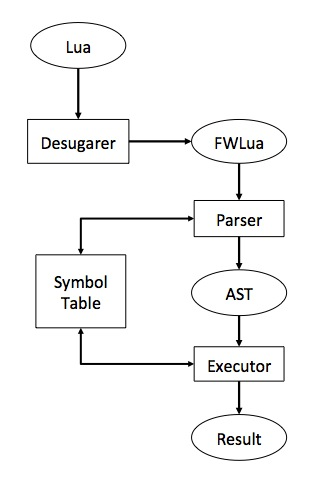
\includegraphics[scale = 0.9]{Interpreter}
\end{figure}
\section{Desugaring in interpreter}
Fortunately, there is a package named {\tt Text.ParserCombinators.Parsec} in Haskell, providing a set of functions for parsing tokens and thus building parsers. We will use this package to build the parser and ``desugarer''. Ref \ref{instrucHAS} shows the detail of this package.

The key role in a functional programming language is recursive functions. Basically, this package allows us to parse token one by one recursively and thus control the data flow. According to this, our method to implement the desugaring is to parse every token in raw code, just like what parser does to code. What is different, this ``desugarer'' will transfer the inputs into another kind of code, instead of making an abstract syntax tree in parser. In other words, the file {\tt desugarer.hs} will take strings as token and then also return strings as new code. For example, we have discussed that the assignment statement in the global environment:
\begin{flushleft}
{\tt x = 42; --In Lua\\
rawset("\_ENV", "x", 42); --equals to in FWLua\\
}
\end{flushleft}
And this is exactly the job of desugarer. Hence for, the code would be like following:
\begin{flushleft}
{\tt 
...\\
assignmentStatement = do\\
~~ident <- identExpression\\
~~spaces\\
~~char '='\\
~~spaces\\
~~val <- expression\\
~~spaces\\
~~return \$ "rawset(" ++ ident ++ ", " ++ val ++ ")"\\
...\\
}
\end{flushleft}

We can see, it will take a set of token with string type, and then return a string as ``new code''. The paradigm of this block would be totally based on the syntactic desugaring methods that we have mentioned in above chapter. The FWLua code this block returns will be used by parser to create AST.

\section{ParserTD.hs}
The structure of parser is similar as desugarer: it uses {\tt parsec} for passing tokens, it takes strings as tokens. The difference is the result it returns is a tree ---- abstract syntax tree (AST).
AST is made up by different type of nodes. Technically, each of these nodes represents a token in the inputs and thus form the whole tree.

In addition, the reason why we call it ``TD'' is because it needs to be asked for parsing inputs from top to down. This order would be very important in programming language. We need to pay attention about this issue, or it will cause several critical problems during being interpreted.

What the parser cares is all about the syntax of FWLua. In other words, there is not any evaluations or storage manipulations in the phase of parsing. The only purpose in this block is to sort the inputs by using the structure of tree, and thus bring the cleaner AST to executer. We can also notice that the AST is completely created by parser. It also means that we can handle different kinds of inputs by using different parsers with the same executor.

\section{Symbol Table}
Haskell is a strong-type programming language. Everything we want to define needs to have a type before we use, and Haskell will strickly follow this type. The tier of symbol table stores all new types we define and it will be used as a user-defined library.

There is two ways declarating new data in Haskell: {\tt data} and {\tt type}. The token {\tt type} allows us to define a new type with single paradigm, while the token {\tt data} defining a new variable type in multiple paradigms with different tokens. For instance, the part of code in symbol tabls is shown:
\begin{flushleft}
{\tt 
type Store = Map Register Table\\
type Argument = String\\
data Value = \\
~~~~VNil\\
~~| VArg String\\
~~| VFunc Argument Expression\\
~~| VResFunc String\\
~~| VReg Register\\
~~| VInt Integer\\
~~| VBool Bool\\
~~| VStr String\\
~~| VTrue\\
~~| VFalse\\
~~deriving (Show)\\
}
\end{flushleft}
In which the type {\tt Store} and {\tt Argument} have the single typing paradigm. They don't need a specific token to be distinguished. On the contratry, the data {\tt Value} has multiple conditions and thus needs different tokens (such like {\tt VArg}, {\tt VFunc} and {\tt VInt} in the code above) in each condition to be figured out.

\section{Executor.hs}
The file {\tt Executor.hs} represents all the whole semantic of FWLua we have given above. There is a function {\tt evaluate()} as the main function in the file. It takes different kinds of nodes in the AST for evaluating, then return values and manipulated store as the final result. Besides, there are several functions for assiting evaluation rules such like address allocation, key pointing, binary operation application and so on. At the beginning, the global store is suppose to be empty. However, we remain a defult metatable and some reserved funtions in it, thus treat it like the initialization of the program.

\section{Run and Runfile}
We have also built a run file to testify if our interpreter works well. What is more, this little file links all components those we introduced before, hence makes it being an entity. In the run file, we just treat inputs as a string flow. Then it will parse it, execute the AST and finally output the results. The results will include desugared code, detail of AST, summary of store and final results. Since it shows every kind of information we need, we can debug our interpreter due to the outputs from this run file.